\documentclass[tikz, border = 2mm]{standalone}
\usepackage{pgfplots}

\pgfkeys{/pgfplots/Delta Style/.style={
    % scale only axis,
    % grid=major,
    axis equal,
    grid style={dashed, gray!30}, %Uncomment these lines for no grid
    axis lines=middle,
    inner axis line style={=stealth}, %Arrow type
    ultra thick,
    xlabel={\large $x$},
    ylabel={\large $y$},
    cycle list = {black,black!70,black!40,black!10} %Plot colors cycle in grayscale
  }}


\pgfplotsset{compat=1.10}
\usepgfplotslibrary{fillbetween}
\usetikzlibrary{patterns}

\usetikzlibrary{shapes}

\tikzset{My Arrow Style/.style={single arrow, fill=blue!25, anchor=base, align=center,text width=1cm}}
\newcommand{\MyArrow}[2][]{\tikz[baseline] \node [My Arrow Style,#1] {#2};}


\begin{document}
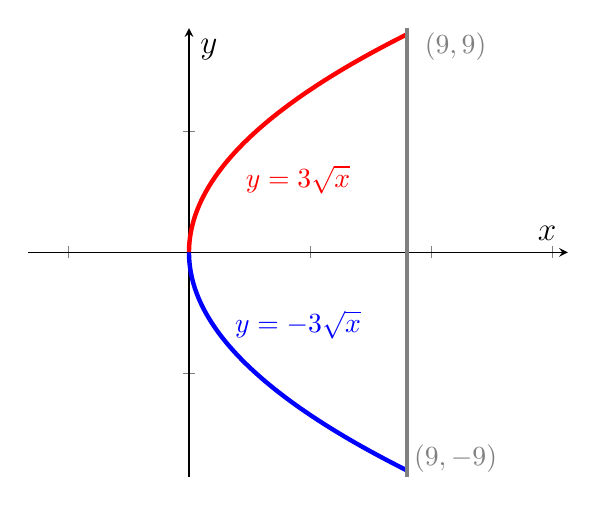
\begin{tikzpicture}
  \begin{axis} [
    Delta Style,
    xmin = -0.25,
    xmax = 9.25,
    ymin = -9.25,
    ymax = 9.25,
    legend pos = south west,
    xticklabels = {$ $,$ $,$ $,$ $,$ $,$ $,$ $,$ $,$ $},
    yticklabels = {$ $,$ $,$ $,$ $,$ $,$ $,$ $,$ $,$ $}
    ]

    \addplot[name path=f,domain = -10:10,ultra thin, opacity=0] (9,x);

    \addplot[name path=axis, domain = -10:10, ultra thin, opacity=0] ({x^2/9},{x});

    \addplot [
        thick,
        color=black,
        fill=blue,
        fill opacity=0.10
    ]
    fill between[
        of=f and axis,
        soft clip={domain=-9:9},
    ];
    
    \addplot [no marks,ultra thick, red, samples=200, domain=0:9] ({x^2/9}, {x});
    \addplot [no marks,ultra thick, blue, samples=200, domain=-9:0] ({x^2/9}, {x});
    \addplot [mark=none,  ultra thick, gray, domain=-10:10] (9,x);
    
    \node[gray] at (axis cs:11,8.5){$(9,9)$};
    \node[gray] at (axis cs:11,-8.5){$(9,-9)$};
    \node[] at (axis cs: 4.5,3){$\textcolor{red}{y=3\sqrt{x}}$};
    \node[] at (axis cs: 4.5,-3){$\textcolor{blue}{y=-3\sqrt{x}}$};

  \end{axis}
\end{tikzpicture}
\end{document}